%%%%%%%%%%%%%%%%%%%%%%%%%%%%%%%%%%%%%%%%%
% Beamer Presentation
% LaTeX Template
% Version 1.0 (10/11/12)
%
% This template has been downloaded from:
% http://www.LaTeXTemplates.com
%
% License:
% CC BY-NC-SA 3.0 (http://creativecommons.org/licenses/by-nc-sa/3.0/)
%
%%%%%%%%%%%%%%%%%%%%%%%%%%%%%%%%%%%%%%%%%

%----------------------------------------------------------------------------------------
%	PACKAGES AND THEMES
%----------------------------------------------------------------------------------------

\documentclass[UTF8,aspectratio=169,14pt]{ctexbeamer}

\usepackage{hyperref}
\hypersetup{
	colorlinks=true,
	linkcolor=red,
	anchorcolor=blue,
	citecolor=green
}

\mode<presentation> {
	
	% The Beamer class comes with a number of default slide themes
	% which change the colors and layouts of slides. Below this is a list
	% of all the themes, uncomment each in turn to see what they look like.
	
	%\usetheme{default}
	%\usetheme{AnnArbor}
	%\usetheme{Antibes}
	%\usetheme{Bergen}
	%\usetheme{Berkeley}
	%\usetheme{Berlin}
	%\usetheme{Boadilla}
	%\usetheme{CambridgeUS}
	%\usetheme{Copenhagen}
	%\usetheme{Darmstadt}
	%\usetheme{Dresden}
	%\usetheme{Frankfurt}
	%\usetheme{Goettingen}
	%\usetheme{Hannover}
	%\usetheme{Ilmenau}
	%\usetheme{JuanLesPins}
	%\usetheme{Luebeck}
	\usetheme{Madrid}
	%\usetheme{Malmoe}
	%\usetheme{Marburg}
	%\usetheme{Montpellier}
	%\usetheme{PaloAlto}
	%\usetheme{Pittsburgh}
	%\usetheme{Rochester}
	%\usetheme{Singapore}
	%\usetheme{Szeged}
	%\usetheme{Warsaw}
	
	% As well as themes, the Beamer class has a number of color themes
	% for any slide theme. Uncomment each of these in turn to see how it
	% changes the colors of your current slide theme.
	
	%\usecolortheme{albatross}
	%\usecolortheme{beaver}
	%\usecolortheme{beetle}
	%\usecolortheme{crane}
	%\usecolortheme{dolphin}
	%\usecolortheme{dove}
	%\usecolortheme{fly}
	%\usecolortheme{lily}
	%\usecolortheme{orchid}
	%\usecolortheme{rose}
	%\usecolortheme{seagull}
	%\usecolortheme{seahorse}
	%\usecolortheme{whale}
	%\usecolortheme{wolverine}
	
	%\setbeamertemplate{footline} % To remove the footer line in all slides uncomment this line
	%\setbeamertemplate{footline}[page number] % To replace the footer line in all slides with a simple slide count uncomment this line
	
	%\setbeamertemplate{navigation symbols}{} % To remove the navigation symbols from the bottom of all slides uncomment this line
}

\usepackage{graphicx} % Allows including images
\graphicspath{{./figs/}}
\usepackage{booktabs} % Allows the use of \toprule, \midrule and \bottomrule in tables
\usepackage{longtable}
\usepackage{listings}
\usepackage{xcolor}
\lstset{numbers=left, %设置行号位置
	numberstyle=\tiny, %设置行号大小
	keywordstyle=\color{blue}, %设置关键字颜色
	commentstyle=\color[cmyk]{1,0,1,0}, %设置注释颜色
	frame=single, %设置边框格式
	escapeinside=``, %逃逸字符(1左面的键),用于显示中文
	%breaklines, %自动折行
	extendedchars=false, %解决代码跨页时,章节标题,页眉等汉字不显示的问题
	xleftmargin=2em,xrightmargin=2em, aboveskip=1em, %设置边距
	tabsize=4, %设置tab空格数
	showspaces=false %不显示空格
}
% Fonts
% \usepackage{libertine}
% \setmonofont{Courier}
\setCJKsansfont[ItalicFont=Noto Serif CJK SC Black, BoldFont=Noto Sans CJK SC Black]{Noto Sans CJK SC}


%----------------------------------------------------------------------------------------
%	TITLE PAGE
%----------------------------------------------------------------------------------------

\title[第1讲]{第12讲 :多处理器调度} % The short title appears at the bottom of every slide, the full title is only on the title page
\subtitle{第三节:O(1) 调度}
\author{向勇、陈渝} % Your name
\institute[清华大学] % Your institution as it will appear on the bottom of every slide, may be shorthand to save space
{
	清华大学计算机系 \\ % Your institution for the title page
	\medskip
	\textit{xyong,yuchen@tsinghua.edu.cn} % Your email address
}
\date{\today} % Date, can be changed to a custom date


\begin{document}

\begin{frame}
\titlepage % Print the title page as the first slide
\end{frame}

%\begin{frame}
%\frametitle{提纲} % Table of contents slide, comment this block out to remove it
%\tableofcontents % Throughout your presentation, if you choose to use \section{} and \subsection{} commands, these will automatically be printed on this slide as an overview of your presentation
%\end{frame}
%
%%----------------------------------------------------------------------------------------
%%	PRESENTATION SLIDES\begin{itemize}
%%----------------------------------------------------------------------------------------
%
%%------------------------------------------------
%\section{第一节:课程概述} % Sections can be created in order to organize your presentation into discrete blocks, all sections and subsections are automatically printed in the table of contents as an overview of the talk
%%------------------------------------------------

% 谈谈调度 - Linux O(1)  https://cloud.tencent.com/developer/article/1077507
% Linux O(1) CPU Scheduler http://people.cs.ksu.edu/~gud/docs/ppt/scheduler.pdf
\begin{frame}
	\frametitle{SMP 和 Linux 内核}
	\begin{columns}
	\begin{column}{.4\textwidth}
	\Large \centering
	
    
\includegraphics[width=1.\textwidth]{single-queue}
	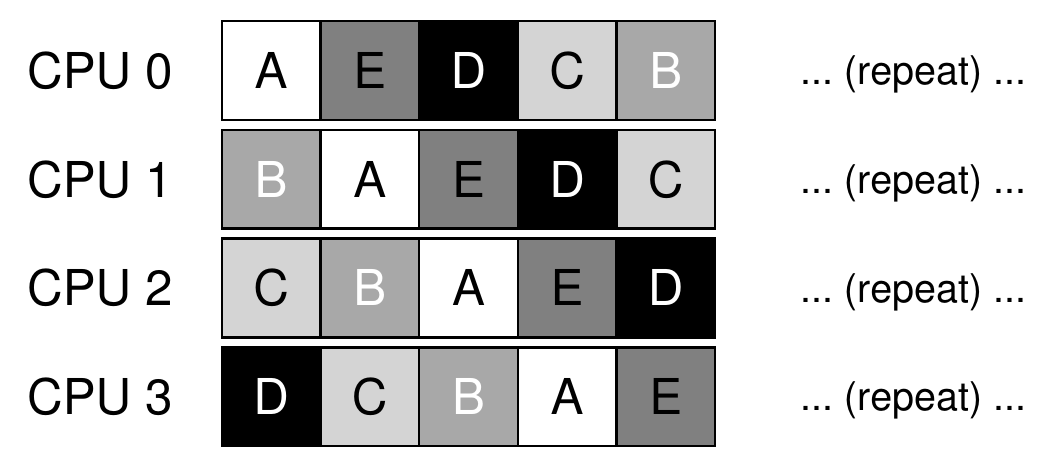
\includegraphics[width=1.\textwidth]{sqms}	
	\end{column}
	
	\begin{column}{.6\textwidth}
%		\large
\begin{itemize}
	\item 在 Linux 2.0 的早期,SMP 支持由一个 “大锁” 组成,这个 “大锁” 对操作系统内部的访问进行串行化
	\item 在2.2前的内核中,SMP实现在用户级,Linux内核本身并不能因为有多个处理器而得到加速

	\end{itemize}

	\end{column}
\end{columns}
\end{frame}


\begin{frame}
	\frametitle{SMP 和 Linux 内核}
	
	\begin{itemize}
		
		\item 在2.4内核后,SMP实现在核心级, 使用多处理器可以加快内核的处理速度。一开始的调度器是复杂度为O(n)的始调度算法
		
		\begin{itemize}
			\item 2.4 scheduler 维护两个 queue:runqueue 和 expired queue
			\item 两个 queue 都永远保持有序
			\item 一个 process 用完时间片,就会被插入 expired queue
			\item 当 runqueue 为空时,只需要把 runqueue 和 expired queue 交换一下即可
		\end{itemize}
	\end{itemize}
	
    \begin{figure}
        \includegraphics[width=0.8\textwidth,natwidth=1011,natheight=343]{figs/linux-2.4-sched.png}
    \end{figure}

\end{frame}

\begin{frame}
	\frametitle{SMP 和 Linux 内核}

	\begin{itemize}
	
	\item 在2.4内核后,SMP实现在核心级, 使用多处理器可以加快内核的处理速度。一开始的调度器是复杂度为O(n)的始调度算法
	
		\begin{itemize}
		\item 全局共享的就绪队列
		\item 寻找下一个可执行的 process,这个操作一般都是 O(1)
		\item 每次进程用完时间片,执行插入操作是,实际上会遍历所有任务,复杂度为O(n)

		\end{itemize}
	\end{itemize}
	
    \begin{figure}
	\includegraphics[width=.8\textwidth]{figs/linux-2.4-sched.png}
    \end{figure}


\end{frame}

\begin{frame}
	\frametitle{SMP 和 Linux 内核}
	
	\begin{itemize}
		
		\item 在2.4内核后,SMP实现在核心级, 使用多处理器可以加快内核的处理速度。一开始的调度器是复杂度为O(n)的始调度算法
		
		\begin{itemize}
			\item 现代操作系统都能运行成千上万个进程
			\item O(n) 算法意味着每次调度时,对于当前执行完的 process,需要把所有在 expired queue 中的 process 过一遍,找到合适的位置插入
			\item 这不仅仅会带来性能上的巨大损失,还使得系统的调度时间非常不确定 —— 根据系统的负载,可能有数倍甚至数百倍的差异
		\end{itemize}
	\end{itemize}
	
    \begin{figure}
    \includegraphics[width=.8\textwidth]{linux-2.4-sched}
    \end{figure}
	
	
\end{frame}
%%------------------------------------------------
\begin{frame}
	\frametitle{ O(1) 调度器}
	\begin{columns}
		\begin{column}{.5\textwidth}
			\Large \centering
			O(1) 调度器
            \begin{figure}
    			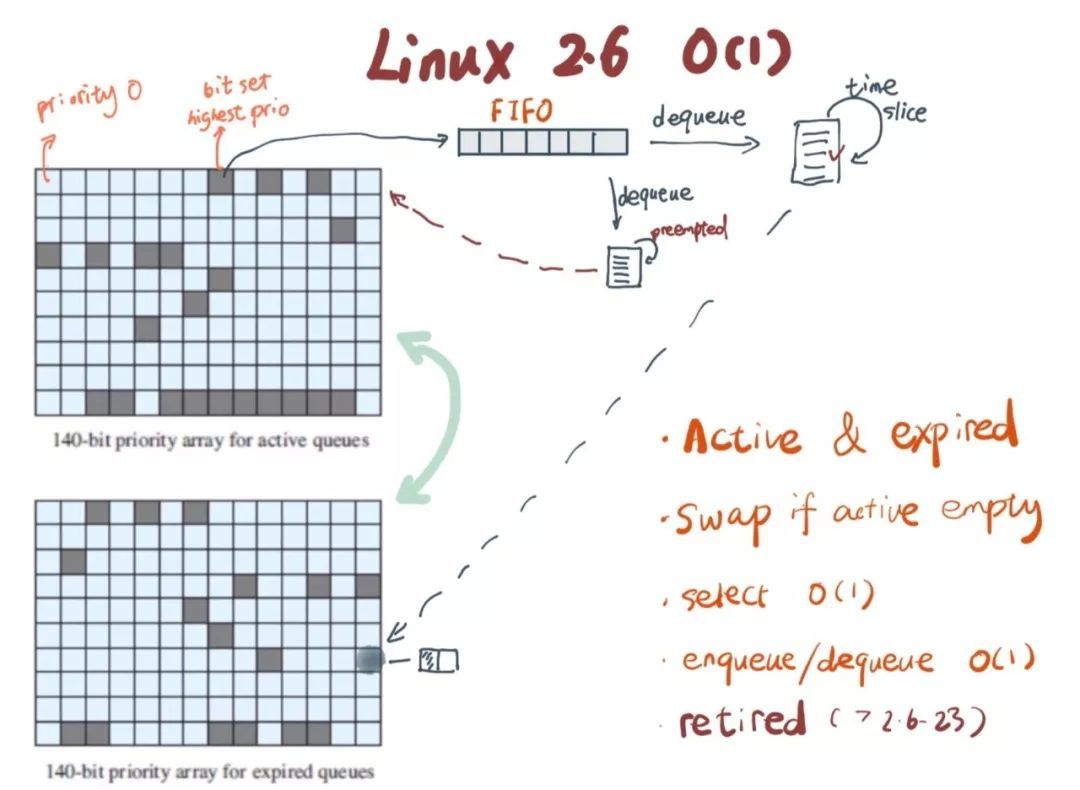
\includegraphics[width=1.\textwidth]{O1}
            \end{figure}
	
		\end{column}
		
		\begin{column}{.5\textwidth}
			\large
			O(1) 调度器 \\
			
2.6 版本的调度器是由 Ingo Molnar 设计并实现的。Ingo 从 1995 年开始就一直参与 Linux 内核的开发。他编写这个新调度器的动机是为唤醒、上下文切换和定时器中断开销建立一个完全 O(1) 的调度器
			
		\end{column}
	\end{columns}
\end{frame}


%%------------------------------------------------
\begin{frame}
	\frametitle{ O(1) 调度器}
	\begin{columns}
		\begin{column}{.4\textwidth}
			\Large \centering
			O(1) 调度器
            \begin{figure}
    			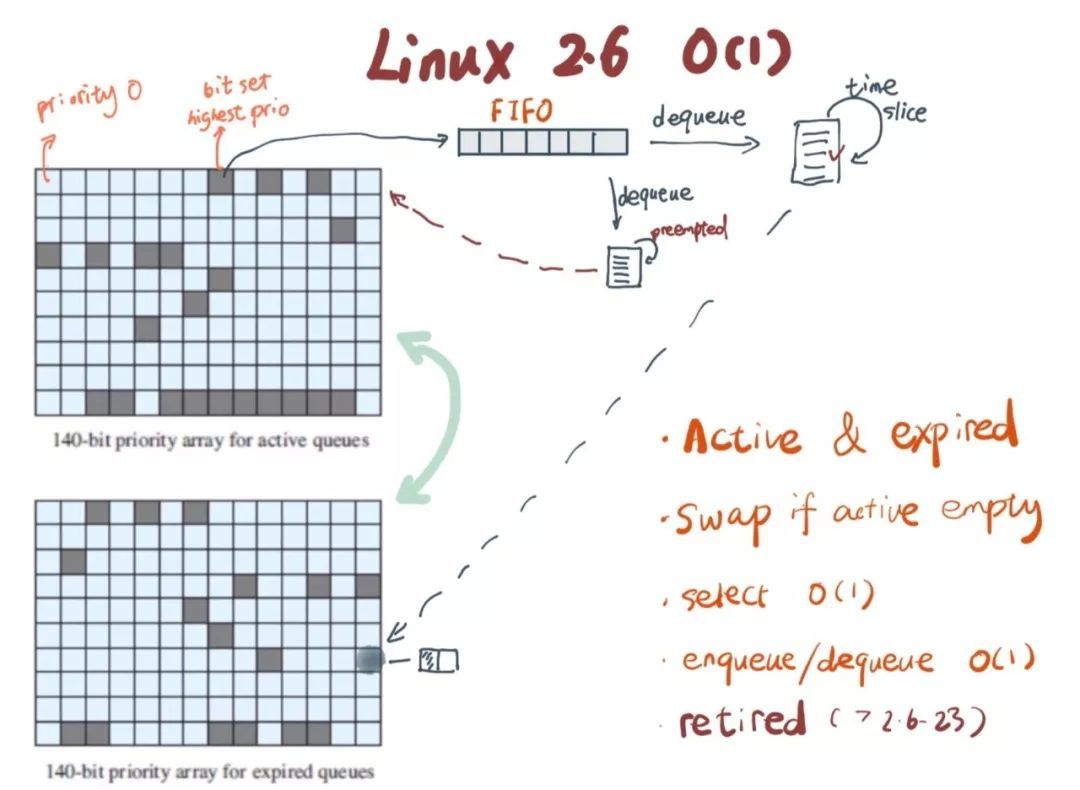
\includegraphics[width=1.\textwidth]{O1}
            \end{figure}
			
		\end{column}
		
		\begin{column}{.6\textwidth}
%			\large
			满足 O(1) 的数据结构?\\
			回顾一下数据结构的四种基本操作和时间复杂度
			\begin{itemize}
			\item access:随机访问
				\begin{itemize}
				\item aarray: 平均情况和最坏情况均能达到 O(1)
				\item linked list 是 O(N)
				\item tree 一般是 O(log N)
				\end{itemize}
			\end{itemize}
		\end{column}
	\end{columns}
\end{frame}


%%------------------------------------------------
\begin{frame}
	\frametitle{ O(1) 调度器}
	\begin{columns}
		\begin{column}{.4\textwidth}
			\Large \centering
			O(1) 调度器
			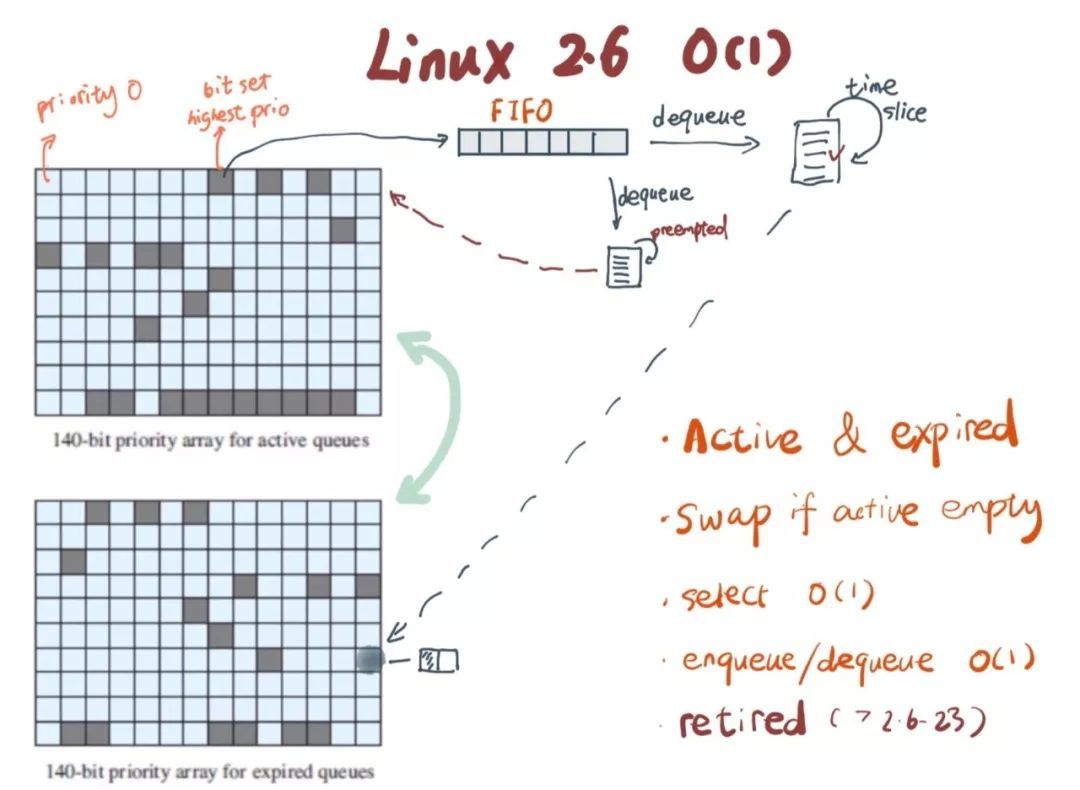
\includegraphics[width=1.\textwidth]{O1}
			
		\end{column}
		
		\begin{column}{.6\textwidth}
			%			\large
			满足 O(1) 的数据结构?\\
			回顾一下数据结构的四种基本操作和时间复杂度
			\begin{itemize}
				\item search:搜索
				\begin{itemize}
					\item hash table 时间复杂度是O(1),但它最坏情况下是 O(N) 
					\item 大部分 tree(b-tree / red-black tree)平均和最坏情况都是 O(log N)
				\end{itemize}
			\end{itemize}
		\end{column}
	\end{columns}
\end{frame}


%%------------------------------------------------
\begin{frame}
	\frametitle{ O(1) 调度器}
	\begin{columns}
		\begin{column}{.4\textwidth}
			\Large \centering
			O(1) 调度器
			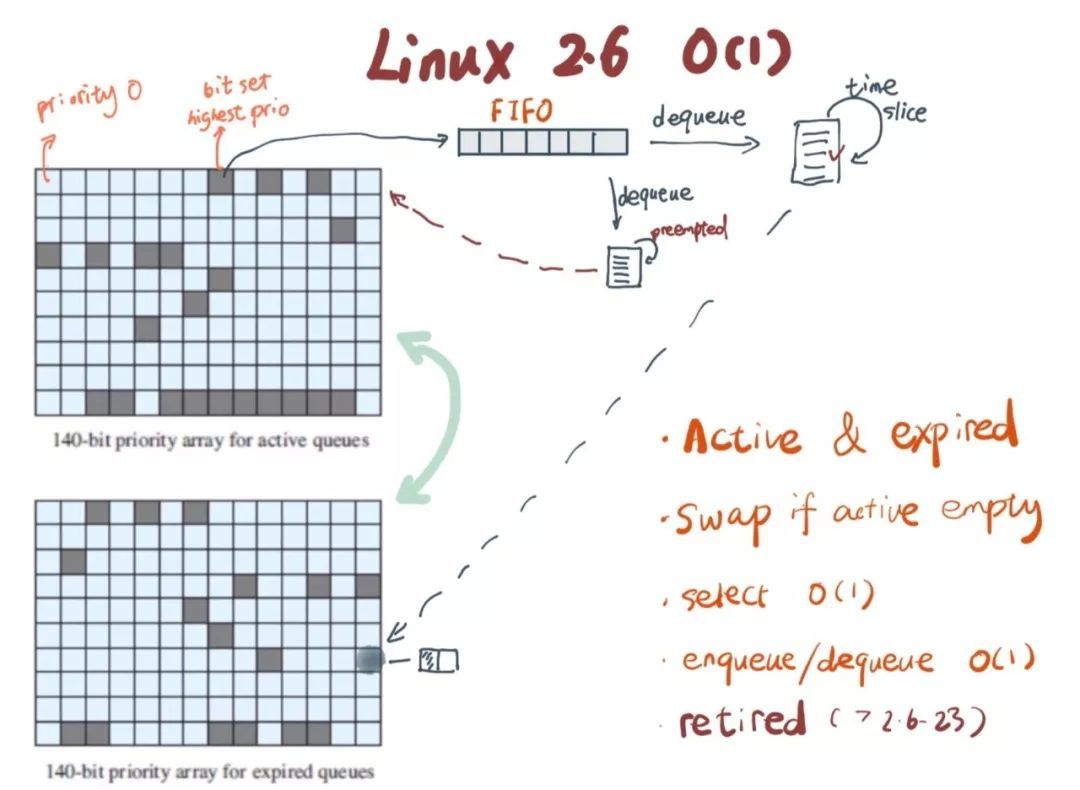
\includegraphics[width=1.\textwidth]{O1}
			
		\end{column}
		
		\begin{column}{.6\textwidth}
			%			\large
			满足 O(1) 的数据结构?\\
			回顾一下数据结构的四种基本操作和时间复杂度
			\begin{itemize}
				\item insert/deletion:插入和删除
				\begin{itemize}
					\item hash table 时间复杂度是O(1),但它最坏情况下是 O(N) 
					\item linked list,stack,queue 在平均和最坏情况下都是 O(1)
				\end{itemize}
			\end{itemize}
		\end{column}
	\end{columns}
\end{frame}



%%------------------------------------------------
\begin{frame}
	\frametitle{ O(1) 调度器}
	\begin{columns}
		\begin{column}{.6\textwidth}
			\Large \centering
			O(1) 调度器
			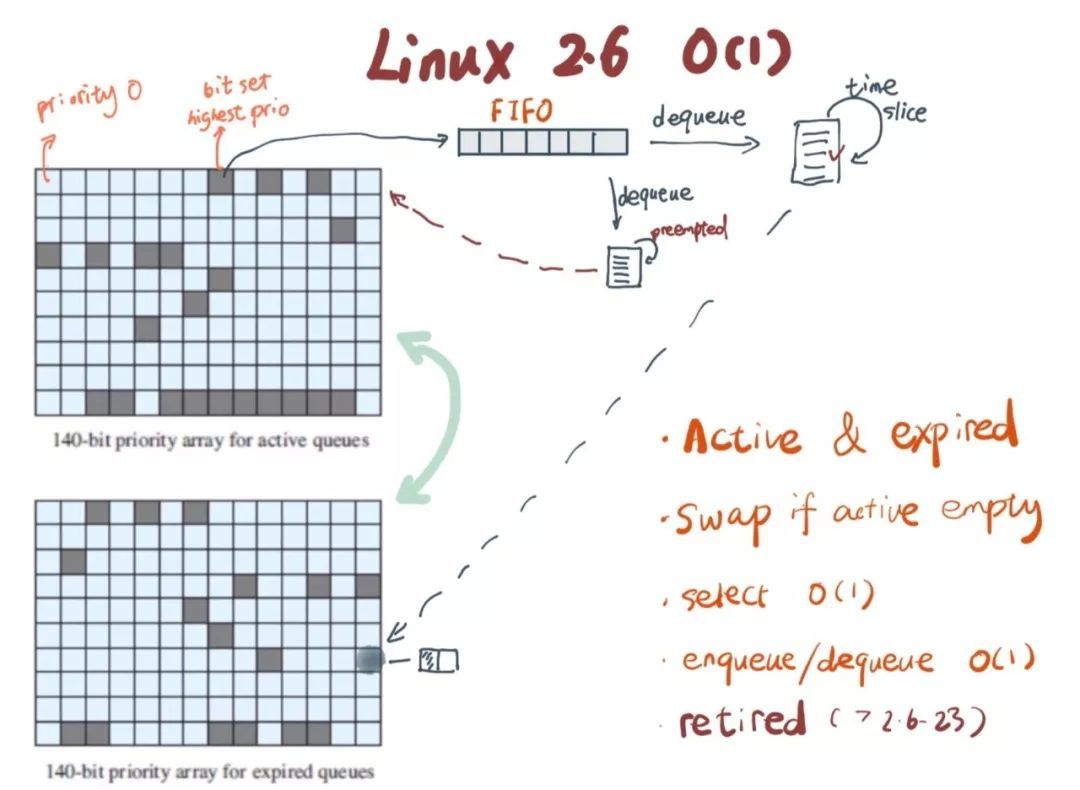
\includegraphics[width=1.\textwidth]{O1-2}
			谈谈调度 - Linux O(1)
		\end{column}
		
		\begin{column}{.4\textwidth}
			%			\large
			O(1) 调度器\\
			
			\begin{itemize}
				\item 进程有140种优先级,可用长度为 140 的 array 去记录优先级。access是O(1)

				\item 每个优先级下面用一个 FIFO queue 管理这个优先级下的 process。新来的插到队尾,先进先出,insert / deletion 都是 O(1)

			\end{itemize}
		\end{column}
	\end{columns}
\end{frame}

%%------------------------------------------------
\begin{frame}
	\frametitle{ O(1) 调度器}
	\begin{columns}
		\begin{column}{.4\textwidth}
			\Large \centering
			O(1) 调度器
			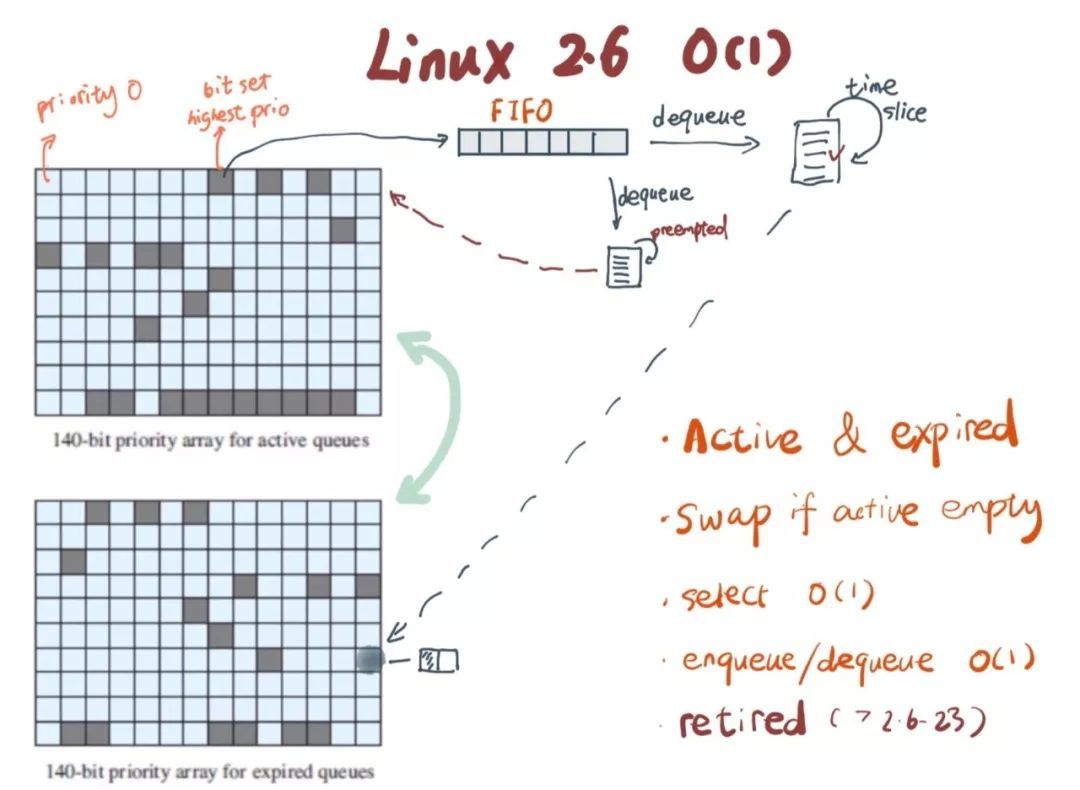
\includegraphics[width=1.\textwidth]{O1-2}
			
		\end{column}
		
		\begin{column}{.6\textwidth}
			%			\large
			O(1) 调度器\\
			
			\begin{itemize}
				\item 进程有140种优先级,可用长度为 140 的 array 去记录优先级。access是O(1)
				
					\begin{itemize}
					\item bitarray,它为每种优先级分配一个 bit,如果这个优先级队列下面有 process,那么就对相应的 bit 染色,置为 1,否则置为 0。
					
					\item 问题就简化成寻找一个 bitarray 里面最高位是 1 的 bit(left-most bit),这基本上是一条 CPU 指令的事。
%					BSR BSF  指令 Intel 80386 https://docs.oracle.com/cd/E19120-01/open.solaris/817-5477/eoizi/index.html
					\end{itemize}
				
			\end{itemize}
		\end{column}
	\end{columns}
\end{frame}

%%------------------------------------------------
\begin{frame}
	\frametitle{ O(1) 调度器}
	\begin{columns}
		\begin{column}{.4\textwidth}
			\Large \centering
			O(1) 调度器
			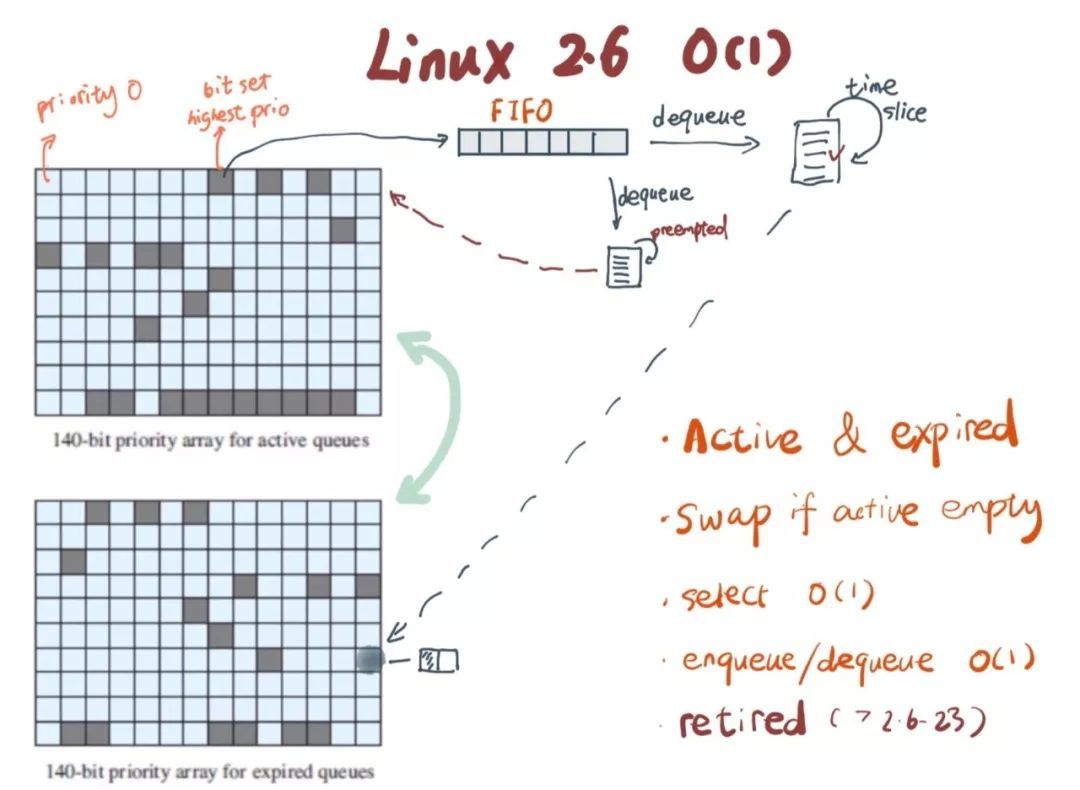
\includegraphics[width=1.\textwidth]{O1-2}
			
		\end{column}
		
		\begin{column}{.6\textwidth}
			%			\large
			O(1) 调度器\\
			
			\begin{itemize}
				\item 在active bitarray(APA)中寻找 left-most bit 的位置 x。
			\item 在APA中找到对应队列 APA[x]。
			\item 从 APA[x] 中 dequeue 一个 process。
			\item 对于当前执行完的 process,重新计算其 priority,然后 enqueue 到 expired priority array(EPA)相应的队里 EPA[priority]。
			\item 如果 priority 在 expired bitarray 里对应的 bit 为 0,将其置 1。
			\item 如果 active bitarray 全为零,将 active bitarray 和 expired bitarray 交换一下。
			\end{itemize}
		\end{column}
	\end{columns}
\end{frame}



%%------------------------------------------------
\begin{frame}
	\frametitle{ O(1) 调度器}
	\begin{columns}
		\begin{column}{.4\textwidth}
			\Large \centering
			O(1) 调度器
			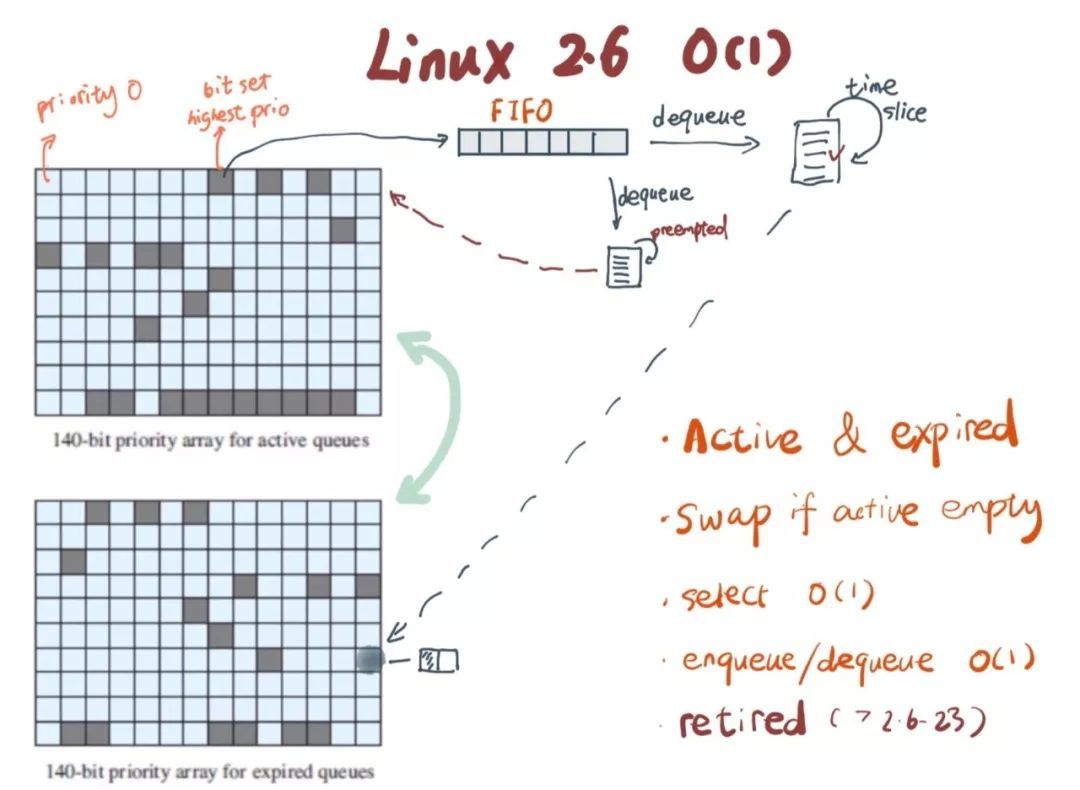
\includegraphics[width=1.\textwidth]{O1-2}
			
		\end{column}
		
		\begin{column}{.6\textwidth}
			%			\large
			O(1) 调度器:多核/SMP支持\\
			
			\begin{itemize}
				\item 在一定时间间隔后,进行load balance分析
				\item  rq­> cpu\_load : represents load on the CPU
				
				\item 在每个时钟中断后进行计算
				\item current\_load = rq­>nr\_running * SCHED\_LOAD\_SCALE;
				
				\item Pulling 进程而不是 pushing进程
				
			\end{itemize}
		\end{column}
	\end{columns}
\end{frame}
%----------------------------------------------
%----------------------------------------------
%----------------------------------------------
\end{document}
